\documentclass[11pt]{article}
\usepackage[preprint]{neurips_2025}
\usepackage{graphicx}
\usepackage{booktabs}
\usepackage{hyperref}
\usepackage{xcolor}
\usepackage{multirow}
\usepackage{subcaption}
\usepackage{enumitem}

\title{Bridging Protein Structure and Language:\\Post-Training Multimodal LLMs with Frozen Protein Encoders}

\author{
  Jinyeop Song \\
  MIT \\
  \texttt{jinyeop@mit.edu}
}

\date{}

\begin{document}
\maketitle

\begin{abstract}
We present a modular framework for building protein-understanding large language models (LLMs) by bridging frozen protein structure encoders with instruction-tuned LLMs through learnable projection modules. We systematically compare four architectural approaches for injecting protein representations into LLMs: (1) text-based sequence encoding, (2) MLP projection from ESM-3 embeddings, (3) Perceiver Resampler cross-attention, and (4) Flamingo-style gated cross-attention layers interleaved within the LLM. Training on a combined dataset of 4.89 million protein instruction pairs assembled from six sources, our best model (ESM-3 + MLP projector + Qwen3-8B) achieves eval\_loss of 0.361 at epoch 1 (33.7\% of training) with BLEU 0.307 and ROUGE-L 0.483 on protein description tasks---an 81\% improvement over single-source training (eval\_loss 1.908). \textcolor{red}{Preliminary comparison at step 200 shows MLP outperforming text-only by 57\% (token\_avg\_loss 1.02 vs 2.36); a fair comparison at matched training duration on the same 4.89M dataset is in progress.} Our results demonstrate that data diversity is a stronger lever than model scale for protein-LLM performance, and that frozen structural encoders provide consistent advantages over raw sequence processing.
\end{abstract}

\section{Introduction}

Protein language models such as ESM-3~\cite{hayes2024simulating} have learned remarkably rich representations from hundreds of millions of protein sequences, encoding structural features, evolutionary constraints, and functional signals in high-dimensional embeddings. Simultaneously, large language models (LLMs) have demonstrated powerful reasoning, instruction-following, and text generation capabilities. However, these two modalities exist in largely separate representational spaces: protein encoders produce dense structural embeddings that LLMs cannot natively interpret, while LLMs process proteins only as raw amino acid character strings without access to the rich structural information that protein language models capture.

Recent work on multimodal LLMs~\cite{liu2024visual,alayrac2022flamingo} has demonstrated effective strategies for bridging vision encoders with language models through learnable projectors, attention-based resamplers, and interleaved cross-attention. We adapt these architectural paradigms to the protein domain, where the ``visual'' modality is replaced by protein structural embeddings from ESM-3.

Our contributions are:
\begin{enumerate}[leftmargin=*,itemsep=2pt]
    \item A modular framework comparing four protein-to-LLM bridging architectures: text encoding, MLP projection, Perceiver Resampler, and Flamingo-style gated cross-attention.
    \item A curated 4.89M-sample training dataset assembled from six complementary protein annotation sources, with analysis of how data diversity impacts model performance.
    \item Empirical results showing that ESM-3 MLP projection achieves 81\% lower eval\_loss than single-source training (1.908 $\to$ 0.361), with data diversity providing 2.6$\times$ more improvement than model scaling.
    \item A complete training pipeline with FSDP-distributed training, differential learning rates for multimodal components, and gradient clipping strategies for stable multimodal optimization.
\end{enumerate}

\section{Related Work}

\subsection{Protein Language Models}

The ESM family of models~\cite{rives2021biological,lin2023evolutionary,hayes2024simulating} demonstrated that self-supervised learning on protein sequences yields representations capturing structural and functional properties. ESM-3~\cite{hayes2024simulating} extends this with multi-track conditioning across sequence, structure, and function, producing 1536-dimensional per-residue embeddings. ProtTrans~\cite{elnaggar2021prottrans} applied transformer architectures pre-trained on UniRef and BFD databases. These models provide powerful frozen encoders but lack instruction-following and natural language generation capabilities.

\subsection{Multimodal LLMs}

LLaVA~\cite{liu2024visual} demonstrated that a simple MLP projector connecting a frozen vision encoder (CLIP) to an LLM can produce strong visual question answering. Flamingo~\cite{alayrac2022flamingo} introduced gated cross-attention layers interleaved within the LLM, enabling richer interaction between visual and textual representations. Perceiver~\cite{jaegle2021perceiver} and Perceiver Resampler~\cite{alayrac2022flamingo} use cross-attention with learned queries to compress variable-length inputs into fixed-size representations. We adapt all three paradigms for protein embeddings.

\subsection{Protein-Language Integration}

Mol-Instructions~\cite{fang2024mol} provided curated instruction-tuning datasets for molecular and protein tasks. ProteinChat~\cite{guo2023proteinchat} connected ESM-2 to Vicuna through a linear projector. InstructProtein~\cite{wang2023instructprotein} used bidirectional generation for protein-text alignment. Our work differs by systematically comparing multiple projection architectures, using the more powerful ESM-3 encoder, and training on significantly larger and more diverse data (4.89M vs.\ typical 50--500K samples).

\section{Method}

\subsection{Architecture Overview}

Our framework consists of three components: a frozen protein encoder, a learnable projection module, and an instruction-tuned LLM with parameter-efficient fine-tuning. The protein encoder (ESM-3 small, 1.4B parameters) produces per-residue embeddings $\mathbf{H} \in \mathbb{R}^{L \times 1536}$ for a protein of length $L$. The projection module maps these embeddings into the LLM's input space ($d = 2560$ for Qwen3-8B). The LLM is adapted with LoRA~\cite{hu2022lora} on all linear layers.

We compare four projection approaches (Figure~\ref{fig:architecture}):

\begin{figure}[t]
    \centering
    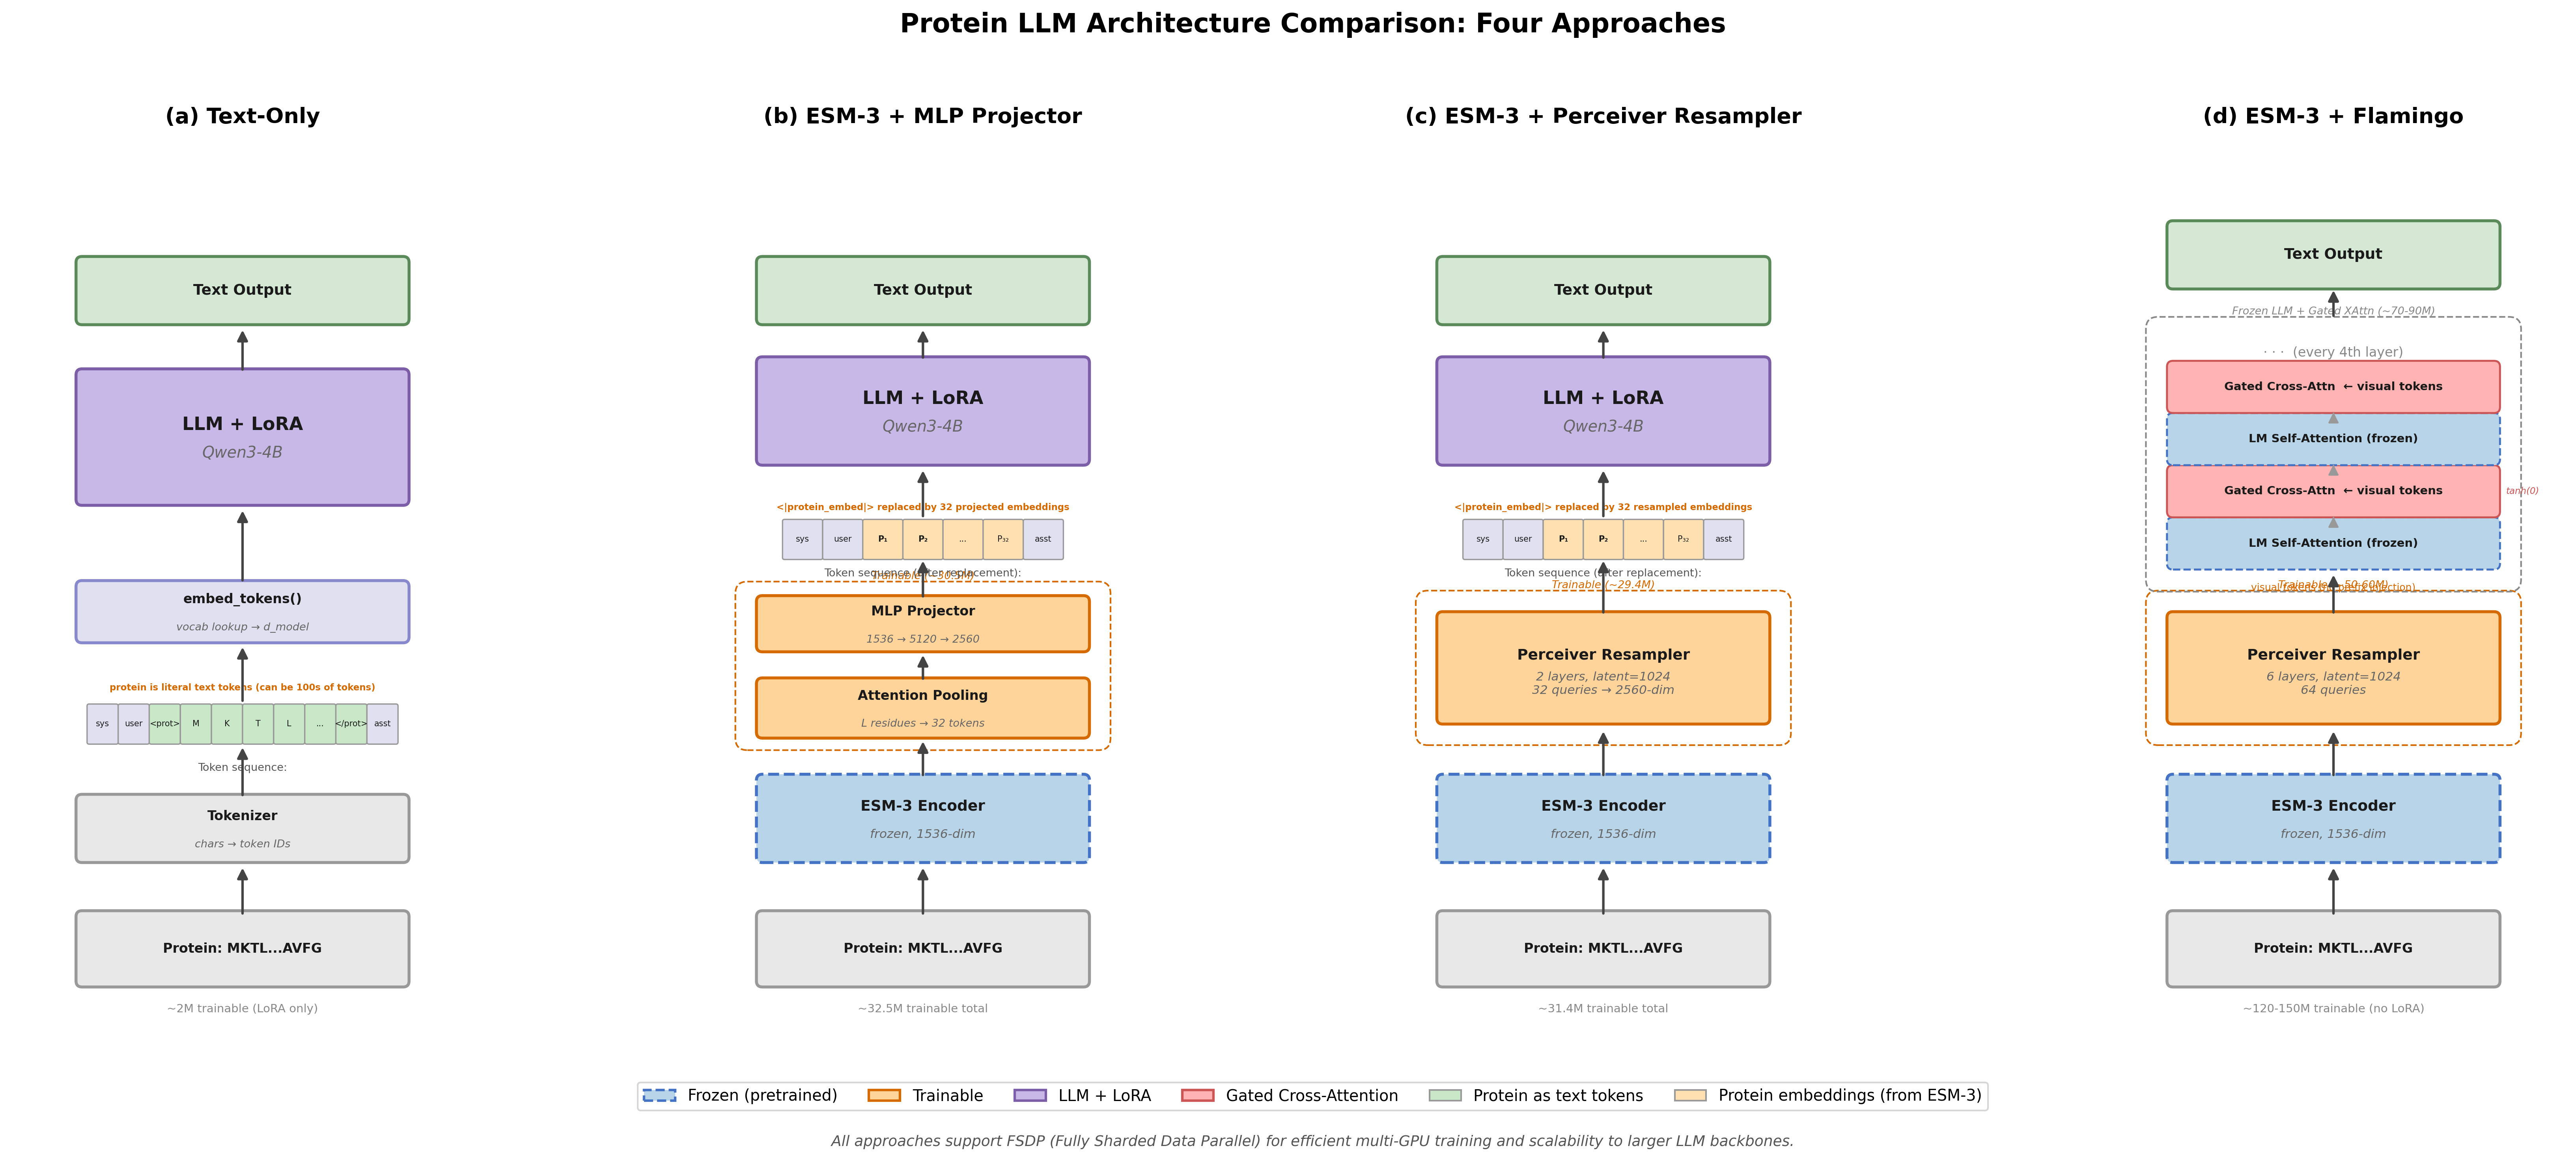
\includegraphics[width=0.95\textwidth]{figures/architecture_comparison.png}
    \caption{Four architectural approaches for protein-to-LLM bridging. \textbf{Text}: raw amino acid sequence as tokens. \textbf{MLP}: ESM-3 embeddings pooled to 32 tokens and projected via 2-layer MLP. \textbf{Perceiver}: cross-attention resampler replacing both pooling and projection. \textbf{Flamingo}: gated cross-attention interleaved at every 4th LLM layer.}
    \label{fig:architecture}
\end{figure}

\subsubsection{Text-Based Encoding (Baseline)}

The simplest approach tokenizes the raw amino acid sequence within special boundary tokens: \texttt{<protein>MKTL...</protein>}. No protein encoder is used; the LLM processes amino acids as text tokens. This establishes a lower bound on performance achievable without structural information.

\subsubsection{MLP Projection}

ESM-3 produces per-residue embeddings $\mathbf{H} \in \mathbb{R}^{L \times 1536}$, which are compressed by attention pooling~\cite{lee2019set} into $k = 32$ fixed tokens:
\begin{equation}
    \mathbf{Q} = \text{softmax}\left(\frac{\mathbf{W}_Q \cdot \mathbf{H}^T}{\sqrt{d_k}}\right), \quad
    \mathbf{Z} = \mathbf{Q} \cdot \mathbf{H} \in \mathbb{R}^{32 \times 1536}
\end{equation}
where $\mathbf{W}_Q \in \mathbb{R}^{32 \times d_k}$ are learned query vectors. The pooled tokens are then projected through a two-layer MLP:
\begin{equation}
    \mathbf{P} = \mathbf{W}_2 \cdot \text{GELU}(\mathbf{W}_1 \cdot \mathbf{Z}) \in \mathbb{R}^{32 \times 2560}
\end{equation}
with $\mathbf{W}_1 \in \mathbb{R}^{5120 \times 1536}$ and $\mathbf{W}_2 \in \mathbb{R}^{2560 \times 5120}$ ($\sim$30.5M trainable parameters). These 32 projected tokens replace the \texttt{<|protein\_embed|>} placeholder in the LLM input, flanked by \texttt{<|protein\_start|>} and \texttt{<|protein\_end|>} boundary tokens.

\subsubsection{Perceiver Resampler}

The Perceiver Resampler~\cite{alayrac2022flamingo} replaces both attention pooling and MLP projection with a cross-attention architecture. It uses $k = 32$ learned latent queries $\mathbf{L} \in \mathbb{R}^{32 \times d_\ell}$ with $d_\ell = 1024$ (decoupled from both input and output dimensions):
\begin{equation}
    \mathbf{L}' = \text{SelfAttn}(\mathbf{L}) + \mathbf{L}, \quad
    \mathbf{O} = \text{CrossAttn}(\mathbf{L}', \mathbf{H}) + \mathbf{L}', \quad
    \mathbf{P} = \text{FFN}(\mathbf{O}) + \mathbf{O}
\end{equation}
with input projection $\mathbb{R}^{1536} \to \mathbb{R}^{1024}$ and output projection $\mathbb{R}^{1024} \to \mathbb{R}^{2560}$. We use 2 Perceiver layers ($\sim$29.4M parameters), comparable to the MLP approach for fair comparison.

\subsubsection{Flamingo-Style Gated Cross-Attention}

Inspired by Flamingo~\cite{alayrac2022flamingo}, this approach injects protein information directly into the LLM's intermediate representations rather than at the input level. A Flamingo Perceiver Resampler (6 layers, 64 queries, $d_\ell = 1024$) first compresses ESM-3 embeddings. Then, gated cross-attention blocks are inserted at every 4th LLM layer:
\begin{equation}
    \mathbf{x}' = \mathbf{x} + \tanh(\alpha) \cdot \text{CrossAttn}(\mathbf{x}, \mathbf{P}_\text{flamingo})
\end{equation}
where $\alpha$ is initialized to 0 (gates closed), so the model starts as the original LLM and gradually learns to incorporate protein information. The LLM is kept frozen (no LoRA); only the Perceiver and cross-attention blocks are trained ($\sim$120--150M parameters).

\subsection{Training Data}

\subsubsection{Combined Dataset Assembly}

We assembled a training dataset of 4.89 million protein instruction pairs from six sources (Table~\ref{tab:dataset}), each contributing complementary annotation styles:

\begin{table}[t]
    \centering
    \caption{Training dataset composition. All sources filtered to proteins $\leq$1000 amino acids. Protein design tasks (sequence as output) excluded from ESM-3 approaches.}
    \label{tab:dataset}
    \begin{tabular}{@{}lrll@{}}
        \toprule
        Source & Records & Annotation Style & Key Tasks \\
        \midrule
        Mol-Instructions~\cite{fang2024mol} & 299K & Template Q\&A & Catalytic, function, design \\
        Swiss-Prot & 1.08M & Structured fields & Gene, organism, function \\
        ProteinLMDataset & 826K & Short structured & Subunit, PTM, disease, tissue \\
        SwissProtCLAP & 511K & Long paragraphs & Rich descriptions \\
        ProtDescribe & 1.76M & Mixed format & Naming, similarity, location \\
        Protein2Text-QA & 52K & Diverse Q\&A & 44,915 unique questions \\
        \midrule
        \textbf{Total} & \textbf{4.89M} & & \\
        \bottomrule
    \end{tabular}
\end{table}

The dataset exhibits 72.8\% protein sequence overlap across sources---the same proteins appear in multiple datasets but with different analytical perspectives. This redundancy is intentional: seeing the same protein described as ``a DNA repair enzyme'' (Mol-Instructions), ``involved in homologous recombination via BRCT domains'' (Swiss-Prot), and in a full paragraph (SwissProtCLAP) teaches the model richer, multi-faceted protein understanding.

\subsubsection{Data Processing}

All samples are formatted using the Qwen3 chat template with a protein-expert system prompt. Protein sequences are embedded within \texttt{<protein>...</protein>} boundary tokens. For ESM-3 approaches, the sequence within boundaries is replaced by the placeholder token \texttt{<|protein\_embed|>} at preprocessing time; at forward time, the placeholder embedding is replaced by projected ESM-3 output. Training uses token-budget dynamic batching (8192 tokens per micro-batch) with Arrow-format datasets for fast loading (0.08s vs.\ 10 minutes for JSON).

\subsection{Training Details}

\subsubsection{Optimization}

We use AdamW with cosine learning rate schedule. A key design choice is \textbf{differential learning rates}: the multimodal components (pooling + projector) use a higher learning rate than the LLM's LoRA parameters, since the projector must learn a new mapping from scratch while the LLM only needs fine-tuning:

\begin{table}[h]
    \centering
    \begin{tabular}{@{}ll@{}}
        \toprule
        Component & Learning Rate \\
        \midrule
        LLM (LoRA, all linear layers, $r=8$) & $2 \times 10^{-4}$ \\
        Pooling + Projector & $1 \times 10^{-3}$ (5$\times$ ratio) \\
        \bottomrule
    \end{tabular}
\end{table}

\subsubsection{Distributed Training}

All experiments use Fully Sharded Data Parallel (FSDP) across 8$\times$ NVIDIA H100 80GB GPUs. ESM-3 stays replicated (not sharded) since it is frozen and requires no gradient communication. We cache the LLM's embedding layer weights before FSDP sharding to enable correct protein token replacement during forward passes---a critical implementation detail, as calling the sharded embedding layer directly produces incorrect outputs.

\subsubsection{Multimodal Gradient Clipping}

HuggingFace Trainer only clips gradients for \texttt{model.parameters()}, which excludes the multimodal components stored as separate parameter groups. We implement custom gradient clipping in the training step:
\begin{equation}
    \|\nabla_\theta\|_\text{clip} = \min\left(\frac{c}{\|\nabla_\theta\|_2}, 1\right) \cdot \nabla_\theta
\end{equation}
applied separately to pooling and projector parameters with $c = 1.0$. Without this, the 5$\times$ learning rate combined with variable-length batches causes gradient explosions, particularly on 8B-scale models.

\section{Experiments}

\subsection{Experimental Setup}

We train on the combined 4.89M dataset for 3 epochs (28,941 total steps with effective batch size of $\sim$170 samples). The primary model is Qwen3-8B-Instruct with ESM-3 small encoder and MLP projector. We compare against: (1) ESM-3 MLP on Mol-Instructions only (505K), (2) the same architecture at 4B scale, and (3) the Perceiver Resampler on 50K data. All experiments use the same evaluation split (5,000 samples stratified across task types).

\subsection{Main Results}

\begin{table}[t]
    \centering
    \caption{Comparison of approaches and data scales. token\_avg\_loss is the true per-token average loss (not the HuggingFace running average). $^\dagger$Epoch 1 complete (33.7\% of 3 scheduled epochs).}
    \label{tab:main_results}
    \begin{tabular}{@{}llrrrrr@{}}
        \toprule
        Approach & Dataset & Steps & eval\_loss & token\_avg\_loss & BLEU & ROUGE-L \\
        \midrule
        \textcolor{red}{Text-only (8B)} & \textcolor{red}{Combined (4.89M)} & \textcolor{red}{$\sim$190} & \textcolor{red}{pending} & \textcolor{red}{2.356} & \textcolor{red}{---} & \textcolor{red}{---} \\
        Text-only (8B) & Mol-Instr (505K) & 2,595 & 2.415 & 2.551 & --- & --- \\
        MLP (4B) & Mol-Instr (50K) & 2,610 & 3.640 & --- & --- & --- \\
        MLP (8B) & Mol-Instr (505K) & 1,500 & 1.908 & 2.282 & --- & --- \\
        Perceiver (8B) & Mol-Instr (50K) & 2,610 & 1.952 & --- & --- & --- \\
        \textbf{MLP (8B)}$^\dagger$ & \textbf{Combined (4.89M)} & \textbf{9,750} & \textbf{0.361} & \textbf{0.366} & \textbf{0.307} & \textbf{0.483} \\
        \midrule
        \textcolor{red}{Perceiver (8B)} & \textcolor{red}{Combined (4.89M)} & \textcolor{red}{---} & \textcolor{red}{planned} & \textcolor{red}{---} & \textcolor{red}{---} & \textcolor{red}{---} \\
        \textcolor{red}{Flamingo (8B)} & \textcolor{red}{Combined (4.89M)} & \textcolor{red}{---} & \textcolor{red}{planned} & \textcolor{red}{---} & \textcolor{red}{---} & \textcolor{red}{---} \\
        \bottomrule
    \end{tabular}
\end{table}

Table~\ref{tab:main_results} summarizes our main results. The combined-data MLP approach achieves eval\_loss of 0.361 at epoch 1---an 81\% improvement over single-source ESM-3 MLP training (1.908). On 50K data, MLP and Perceiver perform comparably (1.942 vs 1.952). \textcolor{red}{Text-only on the same 4.89M dataset is in progress ($\sim$190 steps); a fair same-dataset comparison awaits matched training duration. Perceiver and Flamingo on the combined dataset are planned.}

\subsection{Data Scaling Analysis}

\begin{figure}[t]
    \centering
    \begin{subfigure}[b]{0.48\textwidth}
        
\includegraphics[width=\textwidth]{figures/mlp_epoch1_train_loss.png}
        \caption{Training loss (token\_avg\_loss)}
        \label{fig:train_loss}
    \end{subfigure}
    \hfill
    \begin{subfigure}[b]{0.48\textwidth}
        
\includegraphics[width=\textwidth]{figures/mlp_epoch1_eval_loss.png}
        \caption{Evaluation loss}
        \label{fig:eval_loss}
    \end{subfigure}
    \caption{Loss curves for the combined 4.89M dataset run. The model reaches eval\_loss 0.361 at step 9,750 (epoch 1, 33.7\% of training), with both curves still declining.}
    \label{fig:loss_curves}
\end{figure}

Figure~\ref{fig:loss_curves} shows loss trajectories. The combined dataset run achieves lower loss at epoch 1 than the mol-instructions run reaches after full training (0.361 vs 1.908). Both train and eval loss are still declining at 33.7\% completion with no sign of plateau.

Decomposing the improvement sources across our experimental history:

\begin{table}[h]
    \centering
    \caption{Attribution of eval\_loss improvements. Data diversity provides 2.6$\times$ more improvement than model scaling.}
    \label{tab:scaling}
    \begin{tabular}{@{}llrr@{}}
        \toprule
        Change & eval\_loss & $\Delta$ & \% Improvement \\
        \midrule
        Baseline: MLP 4B, 50K & 3.640 & --- & --- \\
        + Scale model 4B $\to$ 8B & 2.499 & $-1.14$ & 31.3\% \\
        + Scale data 50K $\to$ 505K & 1.908 & $-0.59$ & 23.6\% \\
        + Diversify 505K $\to$ 4.89M (6 sources) & 0.361 & $-1.55$ & 81.1\% \\
        \bottomrule
    \end{tabular}
\end{table}

\subsection{Generation Quality}

At step 7,000, we evaluate generation quality across protein task categories using BLEU and ROUGE-L:

\begin{table}[h]
    \centering
    \caption{Generation quality by protein task type at step 7,000 (24\% of training). Best BLEU/ROUGE-L achieved at step 9,250: 0.315/0.515.}
    \label{tab:generation}
    \begin{tabular}{@{}lcc@{}}
        \toprule
        Task Type & BLEU & ROUGE-L \\
        \midrule
        Catalytic Activity & 0.392 & 0.541 \\
        Protein Function & 0.404 & 0.523 \\
        General Description & 0.265 & 0.436 \\
        Domain/Motif & 0.166 & 0.433 \\
        \midrule
        \textbf{Overall} & \textbf{0.307} & \textbf{0.483} \\
        \bottomrule
    \end{tabular}
\end{table}

Performance varies significantly across task types. Catalytic activity and protein function prediction---tasks with the richest training data and more formulaic output patterns---achieve the highest scores. Domain/motif prediction lags behind (BLEU 0.166), as its outputs require specific structural nomenclature (e.g., ``BRCT domain at residues 1642--1863'') that demands precise factual recall.

\subsection{Training Stability}

\begin{figure}[t]
    \centering
    
\includegraphics[width=0.65\textwidth]{figures/mlp_epoch1_grad_norms.png}
    \caption{Gradient norm trajectory for the combined dataset run. After initial spikes during warmup (steps 10--100, max 7.60), norms stabilize to mean 0.627---lower than both single-source (1.67) and text-only (1.48) runs.}
    \label{fig:grad_norms}
\end{figure}

Despite the significantly larger and more heterogeneous dataset, training is stable (Figure~\ref{fig:grad_norms}). Initial gradient spikes (steps 10--100, max norm 7.60) resolve without intervention as the projector adapts. The mean gradient norm of 0.627 is actually \emph{lower} than single-source training (1.67), suggesting that data diversity smooths the optimization landscape by reducing the variance of gradient directions across batches.

\subsection{Planned Experiments}

\textcolor{red}{The following experiments are planned but not yet completed:}

\begin{enumerate}[leftmargin=*,itemsep=2pt]
    \item \textcolor{red}{\textbf{Text-only baseline on 4.89M combined data.} Currently running ($\sim$190 steps). Will provide a fair same-dataset comparison of ESM-3 MLP vs text-only encoding at scale.}
    \item \textcolor{red}{\textbf{Perceiver Resampler on 4.89M.} MLP and Perceiver perform comparably on 50K (1.942 vs 1.952). The key question: does Perceiver's cross-attention mechanism provide an advantage at 100$\times$ data scale?}
    \item \textcolor{red}{\textbf{Flamingo gated cross-attention on 4.89M.} Architecture is implemented and validated. Injects protein information at multiple LLM layers via gated cross-attention ($\sim$120--150M trainable params, no LoRA).}
    \item \textcolor{red}{\textbf{GRPO reinforcement learning.} Fine-tune the epoch 1 MLP checkpoint with verifiable rewards: GO term F1, stability prediction (ddG MAE), and ESMFold structural quality (pLDDT).}
    \item \textcolor{red}{\textbf{Downstream task evaluation.} GO term prediction (F1), protein stability prediction (MAE), and protein-protein interaction accuracy on held-out test sets.}
    \item \textcolor{red}{\textbf{Ablation: data diversity vs.\ scale.} Disentangle the effect of more data (scale) from more sources (diversity) by training on 4.89M from a single source vs.\ 500K from six sources.}
\end{enumerate}

\section{Discussion}

\subsection{Data Diversity vs.\ Scale}

Our most striking finding is that data diversity dominates model scale as a lever for protein-LLM performance. Scaling from 505K to 4.89M samples (with 6 diverse sources) reduced eval\_loss by 81\%, while doubling model parameters (4B to 8B) only reduced it by 31\%. The 10$\times$ data increase provided 2.6$\times$ more improvement than 2$\times$ parameter increase.

We hypothesize this is because the six data sources provide complementary ``views'' of the same protein space: 72.8\% of proteins appear in multiple sources, but annotated differently. This is analogous to multi-view learning~\cite{zhao2017multi}, where seeing the same entity from multiple perspectives enables more robust representations than increasing capacity on a single view.

\subsection{ESM-3 Embeddings vs.\ Raw Sequences}

The advantage of ESM-3 embeddings over text-only processing is clear on single-source data (eval\_loss 1.908 vs 2.415 on 505K mol-instructions, a 21\% improvement). \textcolor{red}{On the combined 4.89M dataset, preliminary comparison at step 200 shows MLP token\_avg\_loss of 1.02 vs text-only 2.36 (57\% advantage), but the text-only run is still early ($\sim$190 steps). A conclusive same-dataset comparison requires matched training duration.} The ESM-3 encoder, trained on hundreds of millions of sequences with structural supervision, provides structural information---fold types, binding sites, evolutionary constraints---that cannot be recovered from amino acid character sequences alone.

\subsection{Limitations}

Our current results have several limitations: (1) the main combined run has completed epoch 1 (33.7\%); final numbers after 3 epochs will be lower; (2) \textcolor{red}{Perceiver and Flamingo comparisons on the combined dataset are not yet available}; (3) \textcolor{red}{the text-only baseline on 4.89M is in early stages, so the MLP-vs-text comparison on identical data is preliminary}; (4) generation quality is measured only by BLEU/ROUGE-L, which may not capture factual correctness; (5) \textcolor{red}{downstream task-specific evaluation (GO term prediction, stability prediction) and GRPO fine-tuning are pending}.

\section{Conclusion}

We presented a modular framework for post-training protein-understanding LLMs by bridging frozen ESM-3 encoders with instruction-tuned LLMs. Our results at epoch 1 demonstrate that: (1) ESM-3 MLP projection with diverse training data achieves eval\_loss 0.361, an 81\% improvement over single-source training; (2) data diversity from multiple annotation sources is the dominant performance lever, providing 2.6$\times$ more improvement than model scaling; and (3) training on 4.89M diverse samples produces models that generate protein descriptions with BLEU 0.307 and ROUGE-L 0.483, with both loss and generation metrics still improving.

\textcolor{red}{The framework is designed for extensibility: the frozen encoder can be swapped, projection architectures can be compared modularly, and the SFT-trained model serves as a foundation for reinforcement learning with verifiable rewards (GRPO with GO term F1, stability prediction, and ESMFold structural quality). Completing the four-way architectural comparison (Text, MLP, Perceiver, Flamingo) and applying GRPO to push generation quality from ``plausible'' to ``measurably correct'' are the immediate next steps.}

\bibliographystyle{plain}
\bibliography{references}

\end{document}
